%%%%%%%% ICML 2019 EXAMPLE LATEX SUBMISSION FILE %%%%%%%%%%%%%%%%%

\documentclass{article}

% Recommended, but optional, packages for figures and better typesetting:
\usepackage{microtype}
\usepackage{graphicx}
\usepackage{subfigure}
\usepackage{booktabs} % for professional tables
\usepackage{algpseudocode}
\usepackage{amsmath}
\usepackage[section]{placeins}

% hyperref makes hyperlinks in the resulting PDF.
% If your build breaks (sometimes temporarily if a hyperlink spans a page)
% please comment out the following usepackage line and replace
% \usepackage{icml2019} with \usepackage[nohyperref]{icml2019} above.
\usepackage{hyperref}

% Attempt to make hyperref and algorithmic work together better:
\newcommand{\theHalgorithm}{\arabic{algorithm}}

% Use the following line for the initial blind version submitted for review:
%\usepackage{icml2019}

% If accepted, instead use the following line for the camera-ready submission:
\usepackage[accepted]{icml2019}

% The \icmltitle you define below is probably too long as a header.
% Therefore, a short form for the running title is supplied here:
\icmltitlerunning{COSE474-2024F: Final Project Report}

\begin{document}

\twocolumn[
\icmltitle{COSE474-2024F: Final Project Report \\
           Traffic Sign Image Classification}

% It is OKAY to include author information, even for blind
% submissions: the style file will automatically remove it for you
% unless you've provided the [accepted] option to the icml2019
% package.

% List of affiliations: The first argument should be a (short)
% identifier you will use later to specify author affiliations
% Academic affiliations should list Department, University, City, Region, Country
% Industry affiliations should list Company, City, Region, Country

% You can specify symbols, otherwise they are numbered in order.
% Ideally, you should not use this facility. Affiliations will be numbered
% in order of appearance and this is the preferred way.
\icmlsetsymbol{equal}{*}

\begin{icmlauthorlist}
\icmlauthor{Matteo Felipe Merz}{}
\end{icmlauthorlist}

%\icmlaffiliation{ku}{Department of Computer Science \& Engineering, Korea University, Seoul, Korea}


%\icmlcorrespondingauthor{the}{myemail@korea.ac.kr}
%\icmlcorrespondingauthor{Eee Pppp}{ep@eden.co.uk}

% You may provide any keywords that you
% find helpful for describing your paper; these are used to populate
% the "keywords" metadata in the PDF but will not be shown in the document
\icmlkeywords{Machine Learning, ICML, CLIP, Classification, Traffic Signs, Fine-tuning}

\vskip 0.3in
]

% this must go after the closing bracket ] following \twocolumn[ ...

% This command actually creates the footnote in the first column
% listing the affiliations and the copyright notice.
% The command takes one argument, which is text to display at the start of the footnote.
% The \icmlEqualContribution command is standard text for equal contribution.
% Remove it (just {}) if you do not need this facility.

%\printAffiliationsAndNotice{} % leave blank if no need to mention equal contribution
%\printAffiliationsAndNotice{\icmlEqualContribution} % otherwise use the standard text.
%\begin{abstract}
%This document provides a basic paper template and submission guidelines.
%Abstracts must be a single paragraph, ideally between 4--6 sentences long.
%Gross violations will trigger corrections at the camera-ready phase.
%\end{abstract}

\section{Introduction}
Traffic sign recognition is a key topic in computer vision. On the road, traffic signs serve multiple important purposes such as regulating speed and warning drivers of potential hazards that lie ahead. Whether in ADAS (Advanced Driver Assistance Systems) or fully autonomous driving, accurate and reliable road sign recognition plays a vital role in ensuring driver safety. Especially warning signs, which inform the driver about potential dangers that lie ahead, are very important for ensuring the safety of the passengers and other road users.

The goal of this project is to achieve high accuracy image classification on a dataset of warning traffic signs. Warning traffic signs are visually highly similar, which complicates the classification process. To overcome this challenge and accomplish a high classification accuracy, a pre-trained model is fine-tuned on the dataset.

This project consists of two parts. Firstly, the preparation of the data for the fine-tuning process. This includes adding textual descriptions to the data points. Secondly, the model is fine-tuned on the dataset. This process includes careful tuning of hyper-parameters and utilizing contrastive learning to improve the model accuracy.


\section{Methods}
The identification of road signs poses multiple particular challenges. Signs are sometimes occluded by greenery or other drivers and their condition can vary due to their age or pollution. The classification should also work independent of the current weather or time of day. However, the highly similar nature of the signs poses the biggest challenge for the classification.

\begin{figure}[h]
    \centering
    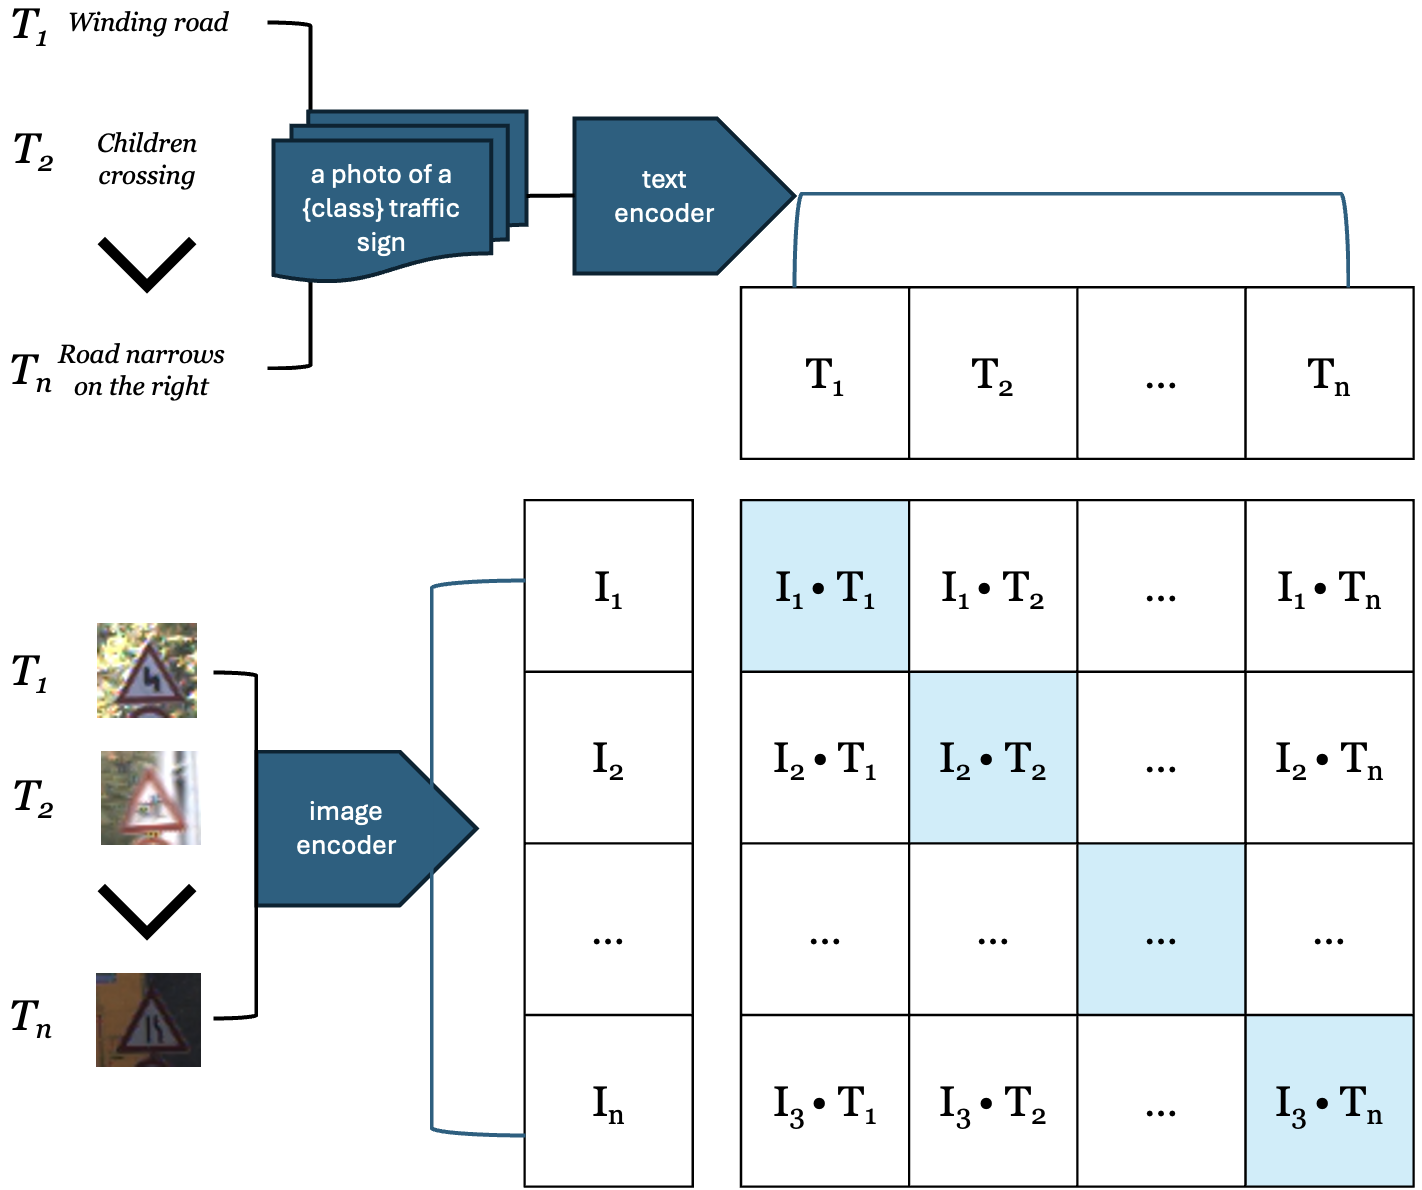
\includegraphics[width=0.9\columnwidth]{images/fine_tune.png}
    \caption{Fine-Tuning Pipeline. The diagonal values are maximized while the other values are minimized.}
    \label{fig:main_figure1}
\end{figure}

\begin{figure}[h]
    \centering
    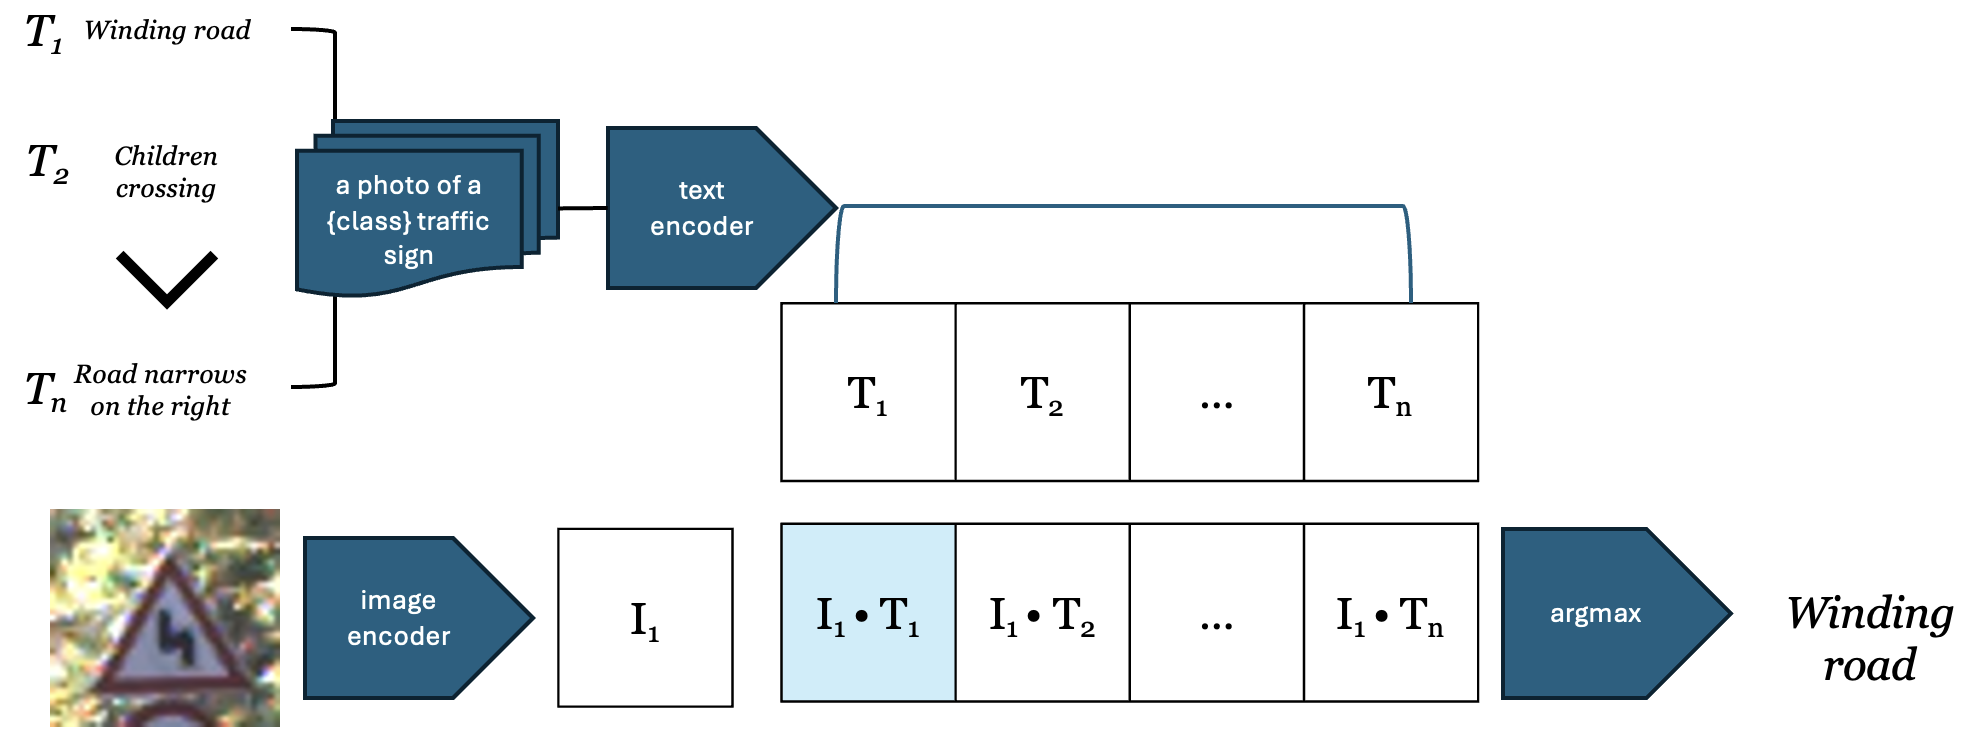
\includegraphics[width=0.9\columnwidth]{images/predict.png}
    \caption{After fine-tuning, an image and all class labels are passed into the encoders. The highest value denotes the inferred class.}
    \label{fig:main_figure2}
\end{figure}

The model used for the image classification is the CLIP (Contrastive Language-Image Pre-Training) model developed by OpenAI. \cite{radford2021learningtransferablevisualmodels} CLIP is a powerful multi-modal model, that connects visual and textual data. It is trained on 400 million text, image pairs and performs especially well in a zero-shot manner. This means that CLIP can even classify images into classes, without being specifically trained on them. While this provides massive benefits for image classification tasks, there are some limitations to CLIP's capabilities. While CLIP can generalize well to common objects, it can struggle with understanding more abstract concepts and very fine-grained classifications. To apply the model in cases, where Zero-Shot classification does not work, the model needs to be fine-tuned to the specific dataset. \cite{goyal2022finetunelikepretrainimproved} Fine-tuning takes advantage of the already pre-trained model and adapts the model weights to better fit the classification task at hand. To achieve this, the model gets trained on the data from the dataset. Fine-tuning can lead to significantly improved performance on highly specialised tasks, while not being as computational intensive as training a model on the data from scratch.

The process for fine-tuning the model is very similar to the initial pre-training of the model. \cite{goyal2022finetunelikepretrainimproved} In each iteration, image and text embeddings are computed for a batch of random pairs from the training data. Based on these embeddings, logits are calculated for both images and text, representing how similar each image is to each piece of text. The loss is calculated by averaging the cross-entropy loss of both directions. As in the pre-training, this encourages the model to maximize the similarity between matching text and image pairs. The resulting model is ready for Inference on the new dataset. The algorithm used for the pre-training of the CLIP model can be found in the Appendix \ref{alg:fine-tune}.

Applying this kind of fine-tuning into the classification of street signs is a novelty, as many fine-tuning solutions only fine-tune CLIP's image encoder and ignore the text encoder entirely. Also using textual descriptions instead of labeled data in the classification of text signs is not very common.
\FloatBarrier
\section{Experiments}
The GTSRB (German Traffic Sign Recognition Benchmark) dataset is used for training and testing the model. \cite{STALLKAMP2012323} In total, the GTSRB contains more than 50,000 images and 40 classes of German traffic signs. It focuses on providing a lifelike database of traffic signs and is therefore well suited for this project. The images in the GTSRB are labeled with a number representing their specific class. For this project 13 classes were selected. They are all warning signs that are commonly used to warn about possible upcoming dangers, like poor road conditions or pedestrians interfering with the flow of traffic. An overview of the classes used in this project can be found in Figure \ref{fig:gtsrb_classes}. The design of these signs is very similar, with all of them being red triangles with graphics indicating the specific danger ahead. Additionally, the traffic signs convey abstract concepts and are probably not part of CLIP's pre-training. This makes accurate zero-shot classification unlikely and highlights the need for fine-tuning.

\begin{figure}[h!]
    \centering
    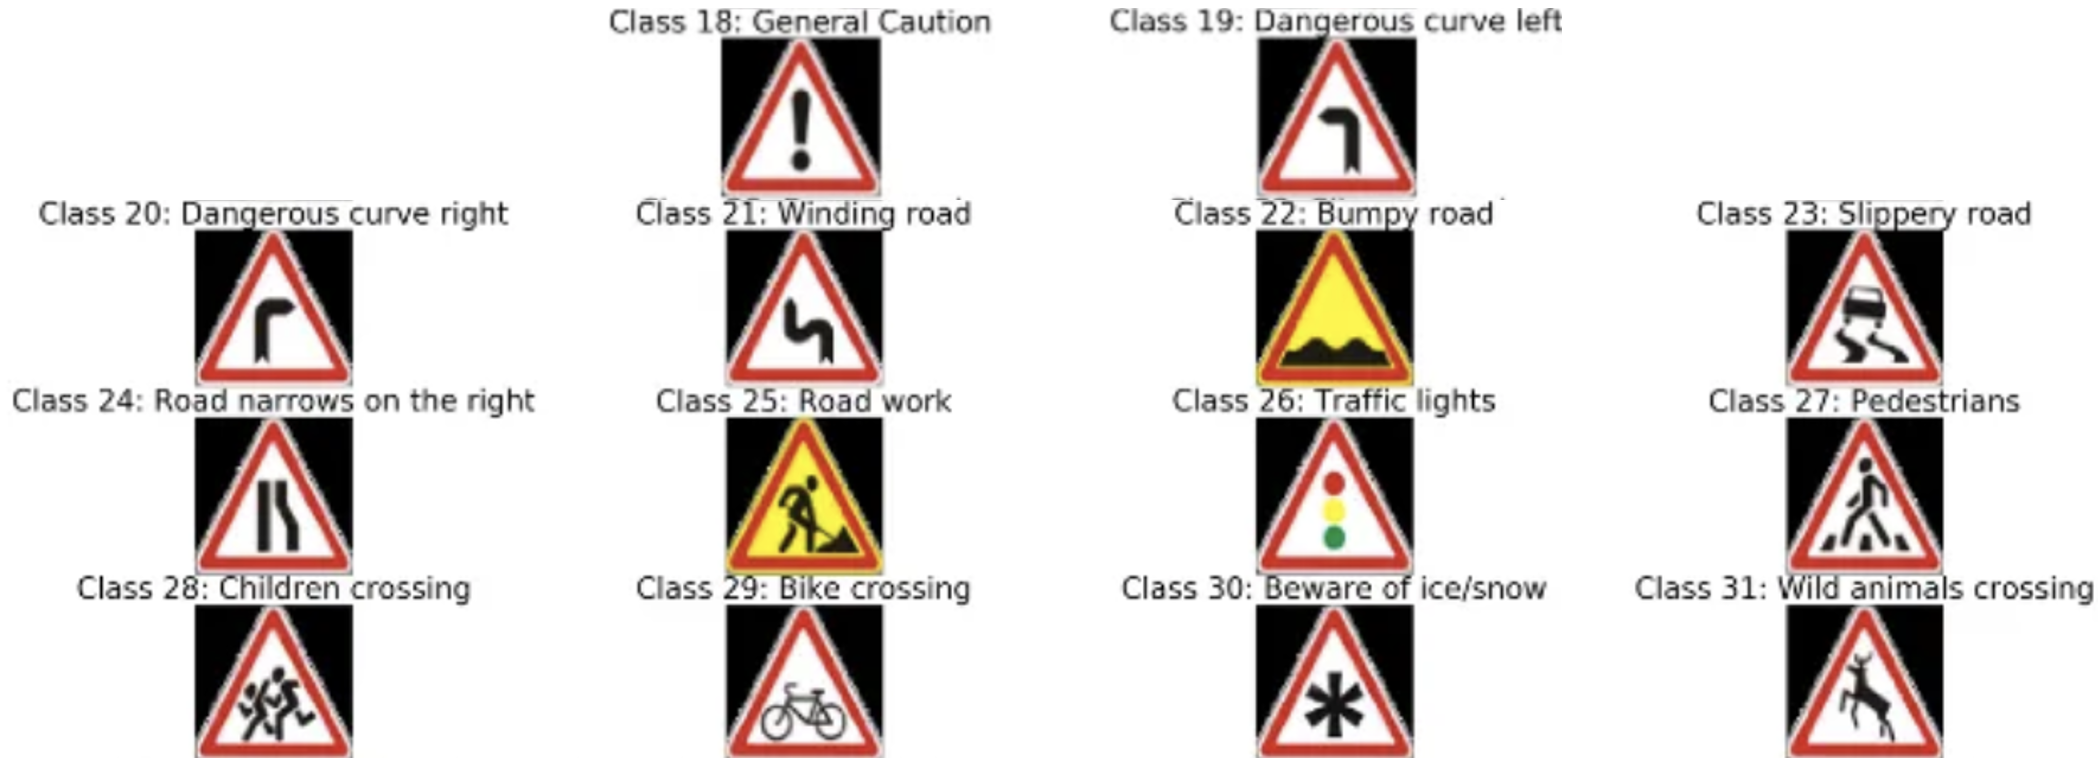
\includegraphics[width=0.9\columnwidth]{images/gtsrb_classes.png}
    \caption{Classes that are used in the image classification.}
    \label{fig:gtsrb_classes}
\end{figure}

The model training and image classification was performed in \citet{GoogleColab}'s web-based Jupyter notebook environment 'Google Colaboratory'. All the computations were performed on a Nvidia T4 GPU. For this project 23 compute units were used in total.

The first step to achieve the image classification is the preparation of the dataset. The GTSRB does not contain text descriptions as class labels and only has a number as the class id associated with each data entry. To leverage the full power of the text and image encoders of the CLIP model, the first step is to map a text description to each of the data points. The description consists of the prefix 'a photo of a ', a short description of the specific danger that the sign is warning about (e.g. 'Children crossing') and the suffix ' traffic sign'. Using natural language descriptions over simple labels, like the name of the class, can evidently lead to increases in model accuracy, as reported by \citet{radford2021learningtransferablevisualmodels}. The next step is the fine-tuning of the model using the technique described in the methods. The optimizer used for the fine-tuning is the AdamW optimizer, which is well suited for fine-tuning CLIP. \cite{loshchilov2019decoupledweightdecayregularization} Through trial and error, a learning rate and a weight decay of 1e-5 were chosen to optimize the learning and reduce over-fitting. The model is only fine-tuned for one epoch as it already reaches a validation accuracy of over 99\% after the first epoch and to limit the computational overhead caused by fine-tuning. 

Before fine-tuning the model, the pre-trained CLIP model reaches an accuracy of around 19.16\% on the test dataset. After fine-tuning for one epoch, the model reaches an accuracy of 94.98\%. Fine-tuning for more epochs can improve this accuracy even further. The improvement highlights the effectiveness of the fine-tuning process. The current state of the art model for the GTSRB, a CNN with three spatial transformers, achieves an accuracy of 99.71\% over all 40 classes of the dataset. \cite{arcos2018deep}

Four random data points were selected from the test dataset to perform a qualitative comparison between the two models. The pre-trained model inferred only one class correctly and chose all classes with a low confidence. This indicates that the model is most likely only guessing the correct class.
\begin{figure}[H]
    \centering
    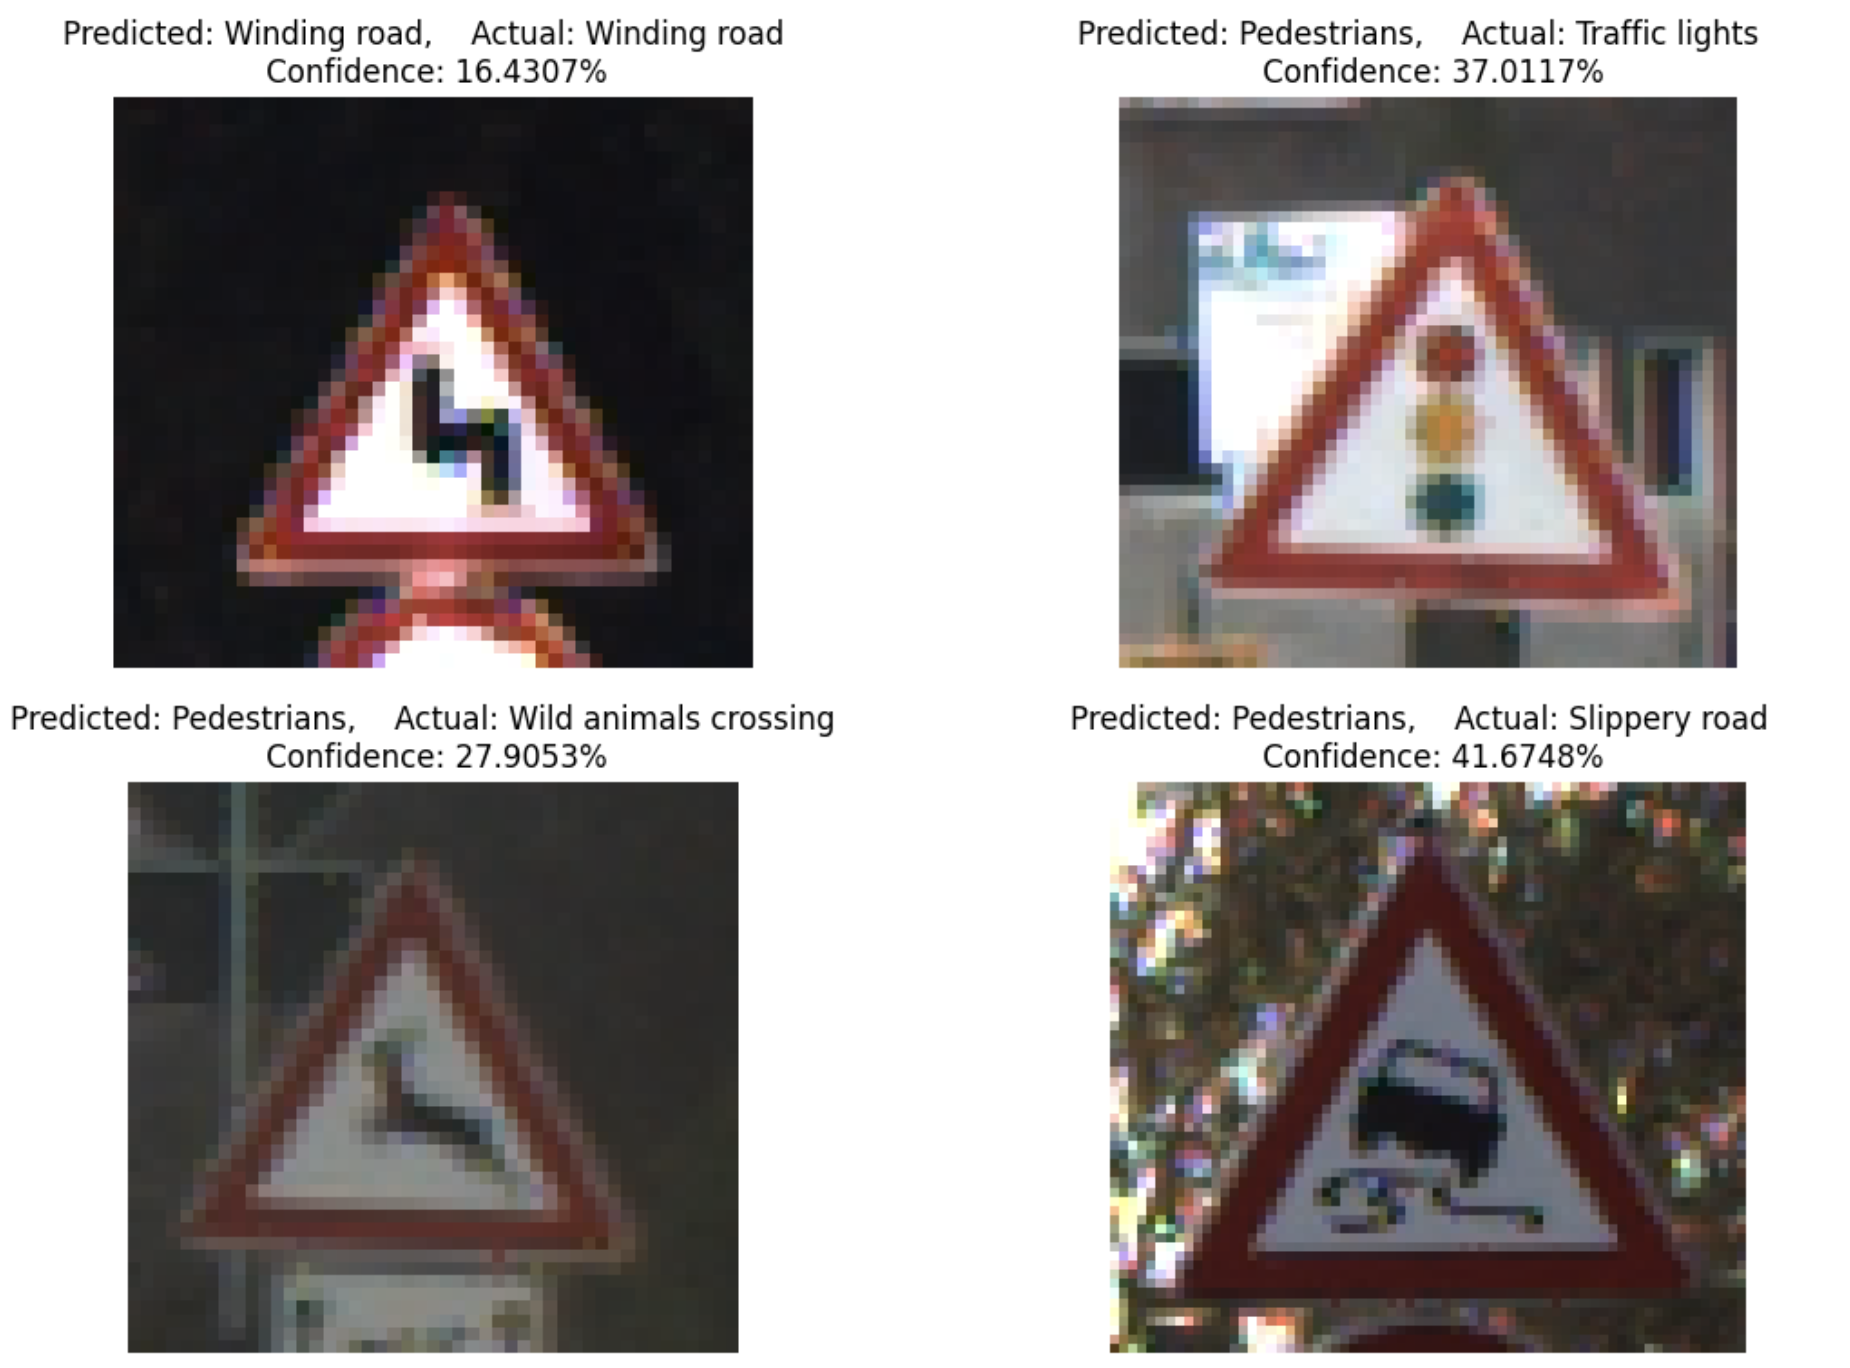
\includegraphics[width=0.9\columnwidth]{images/quali_base.png}
    \caption{Qualitative results of zero-shot image classification.}
    \label{fig:quali_base}
\end{figure}
After the fine-tuning is complete the model correctly infers the right class for every data point and does so with a confidence of over 99\%.
\begin{figure}[H]
    \centering
    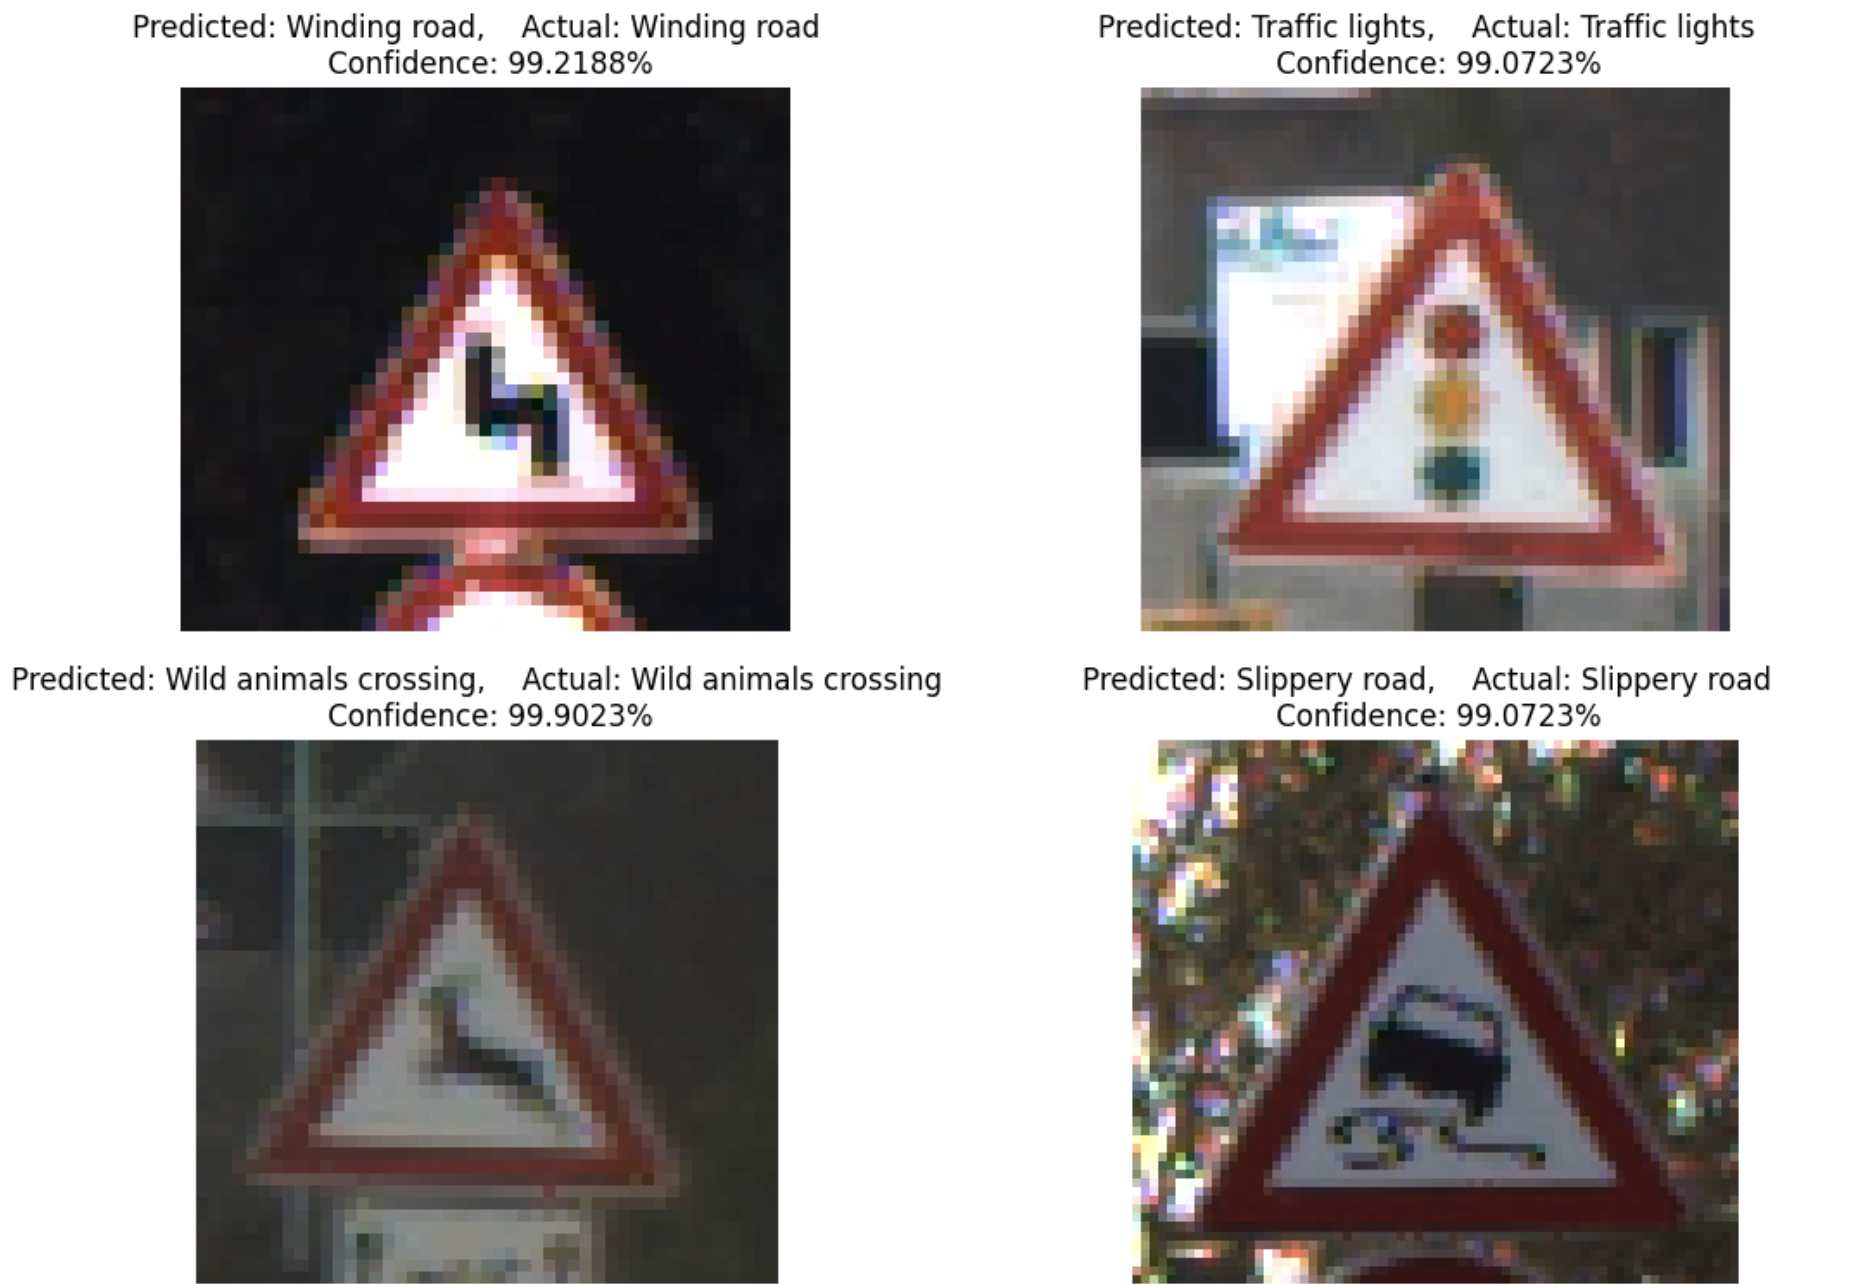
\includegraphics[width=0.9\columnwidth]{images/quali_fine_tuned.png}
    \caption{Qualitative results of image classification using the fine-tuned model.}
    \label{fig:quali_fine}
\end{figure}
In both the comparison of quantitative and qualitative results, the impact of fine-tuning for even a single period on pre-trained models like CLIP can be clearly observed. While the performance of the model does not hold up to the state of the art solution, the achieved accuracy after only one epoch of pre-training is still impressive. Overall, fine-tuning the model achieves the desired high accuracy image classification of the warning traffic signs.

\FloatBarrier
\section{Future Direction}
This project proves the validity and efficiency of the fine-tuning method for adapting a pre-trained model to a specific classification task. One future implication of the results of this study could be the development of an Object Detection model based on the fine-tuned CLIP model. This would enable the detection of multiple warning signs in one traffic scene, which is crucial in real world applications. In the context of this project this direction was also explored, but only with limited success.
\begin{figure}[H]
    \centering
    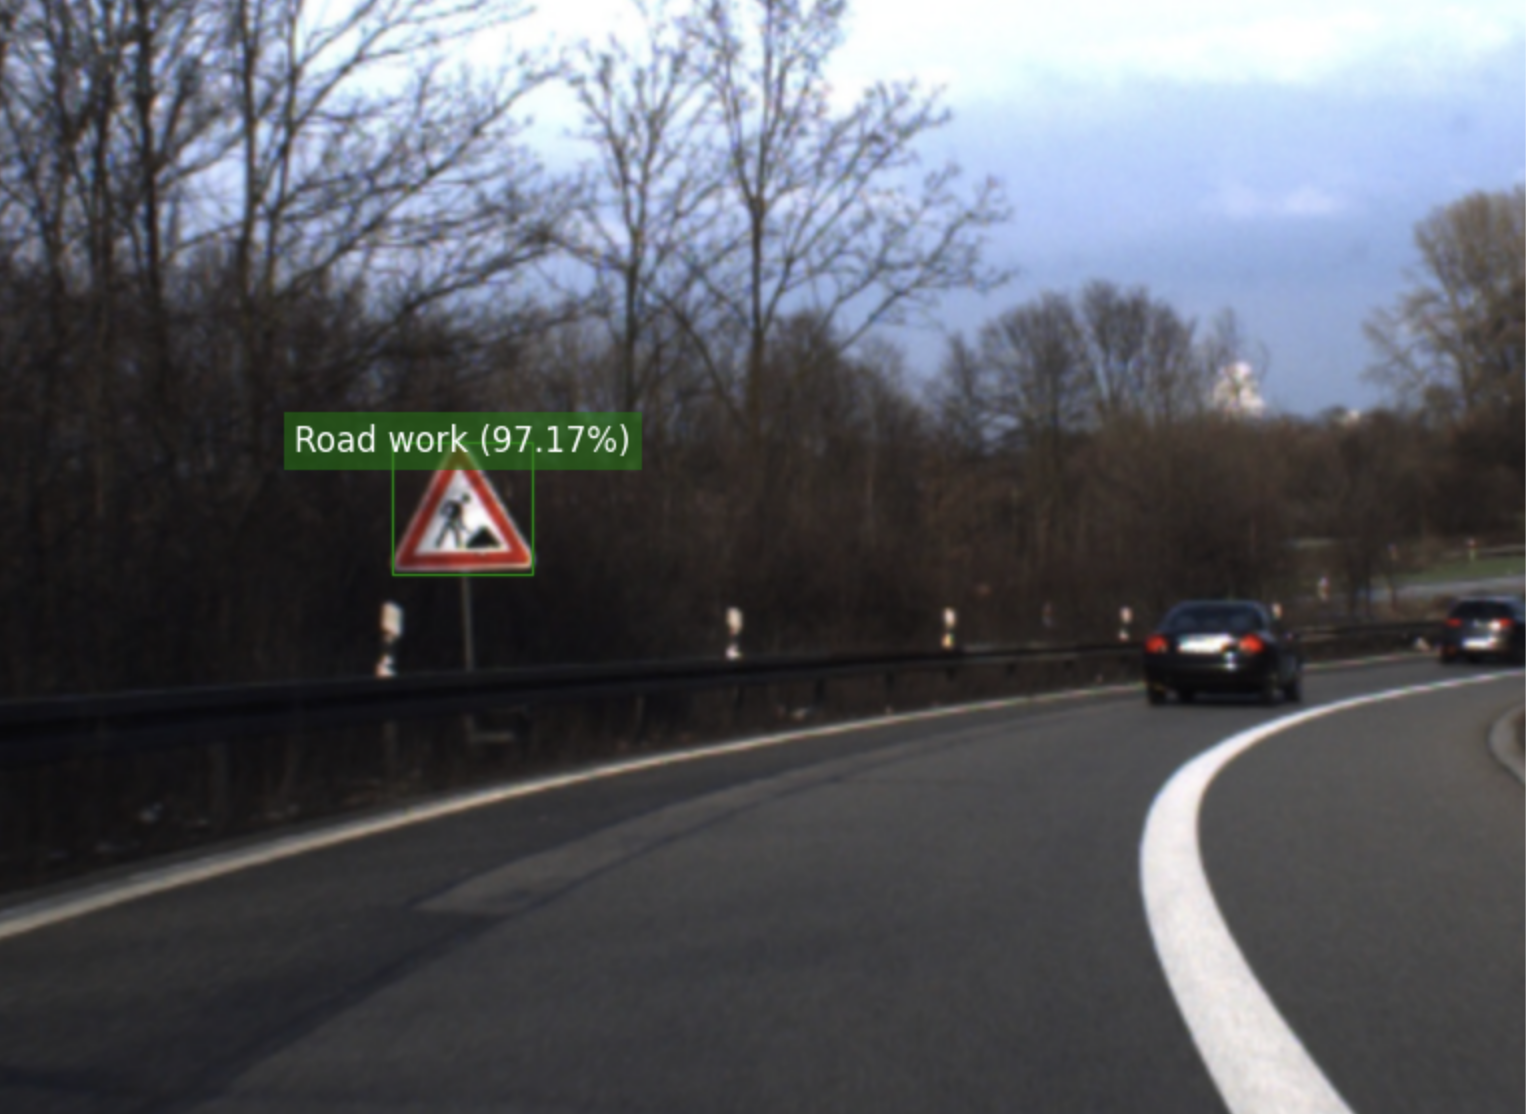
\includegraphics[width=0.7\columnwidth]{images/detection_res.png}
    \caption{Object Detection experiment result conducted with the fine-tuned CLIP model.}
    \label{fig:detection_res}
\end{figure}
Another application of the high accuracy classification would be to combine the detected class label with other objects that are detected in the scene to give specific advice on how the driver should react to be prepared for possible dangerous situations. For example the detection of a person riding a bicycle in combination with a 'Bicycle crossing' sign, could alert the driver to slow down and pay close attention to this specific bike rider. 

\bibliography{report}
\bibliographystyle{icml2019}

\newpage
\appendix
\section{Fine-tuning Algorithm}

%algorithm
\begin{algorithm}[h!]
\caption{Fine-Tuning CLIP on a new dataset}
\begin{algorithmic}[1]
\Require Pre-trained CLIP model, epochs \(E\), dataset \( \mathcal{D} = \{(I_k, T_k)\}_{k=1}^N \), learning rate \(\eta\), 
    temperature \(\tau\), weight decay \( \lambda \)
\Ensure Fine-tuned CLIP model

\State Initialize optimizer \( \text{AdamW}(\theta, \eta, \lambda) \)
\For{epoch \( e \) in \( 1, \dots, E \)}
    \State Shuffle dataset \( \mathcal{D} \)
    \For{each mini-batch \( \mathcal{B} = \{(I_b, T_b)\}_{b=1}^B \) in \( \mathcal{D} \)}
        \State Compute image embeddings \[ Z = \text{ImageEncoder}(I_b) \]
        \State Compute text embeddings \[ W = \text{TextEncoder}(T_b) \]
        
        \State Compute logits for image-to-text: 
        \[
        \text{logits}_{\text{img}} = \frac{Z W^\top}{\tau}
        \]
        \State Compute logits for text-to-image:
        \[
        \text{logits}_{\text{txt}} = \frac{W Z^\top}{\tau}
        \]
        
        \State Set ground truth \( \text{labels} = \{0, \dots, B-1\} \)
        
        \State Compute loss:
        \[
        \mathcal{L}_{\text{img}} = -\frac{1}{B} \sum_{i=1}^B \log \frac{\exp(\text{logits}_{\text{img}}[i, \text{labels}[i]])}{\sum_{j=1}^B \exp(\text{logits}_{\text{img}}[i, j])}
        \]


        \[
        \mathcal{L}_{\text{txt}} = -\frac{1}{B} \sum_{i=1}^B \log \frac{\exp(\text{logits}_{\text{txt}}[i, \text{labels}[i]])}{\sum_{j=1}^B \exp(\text{logits}_{\text{txt}}[i, j])}
        \]
        \[
        \mathcal{L}_{\text{total}} = \frac{\mathcal{L}_{\text{img}} + \mathcal{L}_{\text{txt}}}{2}
        \]
        
        \State Backpropagate loss \( \mathcal{L}_{\text{total}} \)
        \State Update model parameters using \( \text{AdamW} \)
    \EndFor
\EndFor

\State Return fine-tuned CLIP model
\end{algorithmic}
\label{alg:fine-tune}
\end{algorithm}
%algorithm

\section{Project Links}
The project report source files and editing history can be accessed on \href{https://sharelatex.tum.de/project/674fad5f337a99e91b997e9c}{Overleaf}. 

The project repository can be accessed on \href{https://github.com/matteomrz/20242R0136COSE47402/tree/792bd2620450ef04677d07a3e92b6c742aed11cd/final}{GitHub}.

\clearpage

\end{document}


% This document was modified from the file originally made available by
% Pat Langley and Andrea Danyluk for ICML-2K. This version was created
% by Iain Murray in 2018, and modified by Alexandre Bouchard in
% 2019. Previous contributors include Dan Roy, Lise Getoor and Tobias
% Scheffer, which was slightly modified from the 2010 version by
% Thorsten Joachims & Johannes Fuernkranz, slightly modified from the
% 2009 version by Kiri Wagstaff and Sam Roweis's 2008 version, which is
% slightly modified from Prasad Tadepalli's 2007 version which is a
% lightly changed version of the previous year's version by Andrew
% Moore, which was in turn edited from those of Kristian Kersting and
% Codrina Lauth. Alex Smola contributed to the algorithmic style files.
